% % no answer key
% \documentclass[letterpaper]{exam}

% answer key
\documentclass[letterpaper, landscape]{exam}
\usepackage{2in1, lscape} 
\printanswers{}

\usepackage{units} 
\usepackage{parskip} 
\usepackage{xfrac} 
\usepackage[fleqn]{amsmath}
\usepackage{cancel}
\usepackage{float}
\usepackage{mdwlist}
\usepackage{booktabs}
\usepackage{cancel}
\usepackage{polynom}
\usepackage{caption}
\usepackage{fullpage}
\usepackage{comment}
\usepackage{enumerate}
\usepackage{graphicx}
\usepackage{mathtools} 
\usepackage{commath}

% puts commas between thousands with \num{12345667}
\usepackage[group-separator={,}]{siunitx}

\everymath{\displaystyle}

\title{Statistics \\ Week Twelve}
\date{\today}
\author{}

\begin{document}

  \maketitle
  \tableofcontents

  \subsection{Pick a Number}
  Everyone in the class pick a number between 1 and 100. What is the probability
  of at least one match?

  \begin{solution}
    With 15 people, the probability that all the numbers are different is:
    \[
      \frac{100 \cdot 99 \cdot 98 \cdot \ldots}{100^{15}} \approx 0.33
    \]

    The probability of at least one pair is
    \[
      1 - \frac{100 \cdot 99 \cdot 98 \cdot \ldots}{100^{15}} \approx \boxed{ 0.67 }
    \]
  \end{solution}

  \subsection{Examples}


  \subsection{Dogs and Cats}
  \begin{table}[H]
    \begin{tabular}[H]{lrrr}
      \toprule
      species & white & black & total\\
      \midrule
      dog     & 30    & 70    & 100\\
      cat     & 25    & 25    & 50\\
      \midrule
      total   & 45    & 105   & 150\\
      \bottomrule
    \end{tabular}
  \end{table}

  \begin{table}[H]
    \begin{tabular}{rlrrr}
      \toprule
        & species & white  & black  & (all) \\
      \midrule
      1 & dog     & 0.2000 & 0.4667 & 0.6667 \\
      2 & cat     & 0.1667 & 0.1667 & 0.3333 \\
      \midrule
      3 & (all)   & 0.3667 & 0.6333 & 1.0000 \\
      \bottomrule
    \end{tabular}
  \end{table}

  \begin{table}[ht]
    \begin{tabular}{rllr}
      \toprule
         & species & color & proportion \\
      \midrule
      1  & dog     & white & 0.3000 \\
      2  & dog     & black & 0.7000 \\
      \midrule
      3  & cat     & white & 0.5000 \\
      4  & cat     & black & 0.5000 \\
      \bottomrule
    \end{tabular}
  \end{table}

  \begin{table}[ht]
    \begin{tabular}{rllr}
      \toprule
         & color & species & proportion \\
      \midrule
      1  & white & dog     & 0.5455 \\
      2  & white & cat     & 0.4545 \\
      \midrule
      3  & black & dog     & 0.7368 \\
      4  & black & cat     & 0.2632 \\
      \bottomrule
    \end{tabular}
  \end{table}

  What's the probability of a randomly selected animal being a black dog:
  \[
    \frac{70}{150} \approx 0.4667 \\
  \]

  \begin{align*}
    P(\text{black dog}) & = P(\text{dog}) \cdot P(\text{black } | \text{ dog}) \\
                        & = 0.6667 \cdot 0.7 \\
                        & \approx 0.4666 \\
                        \\
    P(\text{black dog}) & = P(\text{black}) \cdot P(\text{dog } | \text{ black}) \\
                        & = 0.6333 \cdot 0.7368 \\
                        & \approx 0.4666 \\
  \end{align*}

  \begin{align*}
    P(\text{black } | \text{ dog}) & = \frac{P(\text{black dog})}{P(\text{dog})} \\
                                   & \approx \frac{0.4667}{0.6667} \\
                                   & = 0.7 \\
  \end{align*}

  \begin{align*}
    P(\text{dog } | \text{ black}) & = \frac{P(\text{black dog})}{P(\text{black})} \\
                                   & \approx \frac{0.4667}{0.7} \\
                                   & = 0.6667 \\
  \end{align*}


  \subsection{Investment Decision}
  Expected value can also help us untangle complex decisions that involve many
  contingencies at different points in time. 

  Suppose a friend of yours has asked you to invest \$1 million in a research
  venture examining a new cure for male pattern baldness. You would probably ask
  what the likelihood of success will be; you’ll get a complicated answer. This
  is a research project, so there is only a 30 percent chance that the team will
  discover a cure that works. If the team does not find a cure, you will get
  \$250,000 of your investment back, as those funds will have been reserved for
  taking the drug to market (testing, marketing, etc.) Even if the researchers
  are successful, there is only a 60 percent chance that the U.S. Food and Drug
  Administration will approve the new miracle baldness cure as safe for use on
  humans. Even then, if the drug is safe and effective, there is a 10 percent
  chance that a competitor will come to market with a better drug at about the
  same time, wiping out any potential profits. If everything goes well---the drug
  is safe, effective, and unchallenged by competitors---then the best estimate
  on the return on your investment is \$ 25 million. 

  Should you make the investment? 

  % This seems like a muddle of information. The potential payday is huge— 25 times
  % your initial investment— but there are so many potential pitfalls.  A decision
  % tree can help organize this kind of information and— if the probabilities
  % associated with each outcome are correct— give you a probabilistic assessment of
  % what you ought to do. The decision tree maps out each source of uncertainty and
  % the probabilities associated with all possible outcomes. The end of the tree
  % gives us all the possible payoffs and the probability of each. If we weight each
  % payoff by its likelihood, and sum all the possibilities, we will get the
  % expected value of this investment opportunity. As usual, the best way to
  % understand this is to take a look.

  \begin{figure}[H]
    \centering
    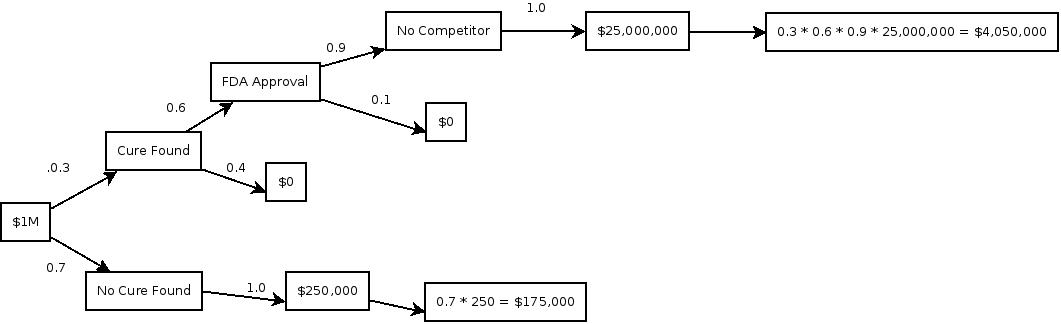
\includegraphics[scale = 0.25]{investment.jpeg}
    \caption{Investment Decision}
  \end{figure}

  \begin{solution}
    \begin{itemize*}
      \item There is a 0.7 chance of \$175,000 
      \item There is a 0.162 chance of \$4,050,000 
      \item There is a 0.138 chance of \$0
    \end{itemize*}
    
    \$4,050,000 + \$175,000 = \fbox{ \$4,225,000 }

    It's a good investment, as long as you can afford to invest in enough
    companies for the law of large numbers to take effect.

   \end{solution}

\end{document}

